%Entities
\section{Entities and their Relationships}

The first step for the development of the new JAQPOT Quattro
platform is to savy the essential entities of the project
and their relationships.
The ER sketch of JAQPOT Quattro is inspirited by the OpenTox
ontology and is concisely presented in the next figure.

\subsection{User}
JAQPOT stores some very basic information about users so as to
manage users' quota. Users have identifying information such as 
their email and name, and a list of limitations (if any) such 
as the maximum number of parallel tasks they can run on the system,
the maximum number of models they may store, datasets to create and
so on.

\begin{figure}[h]
 \centering
 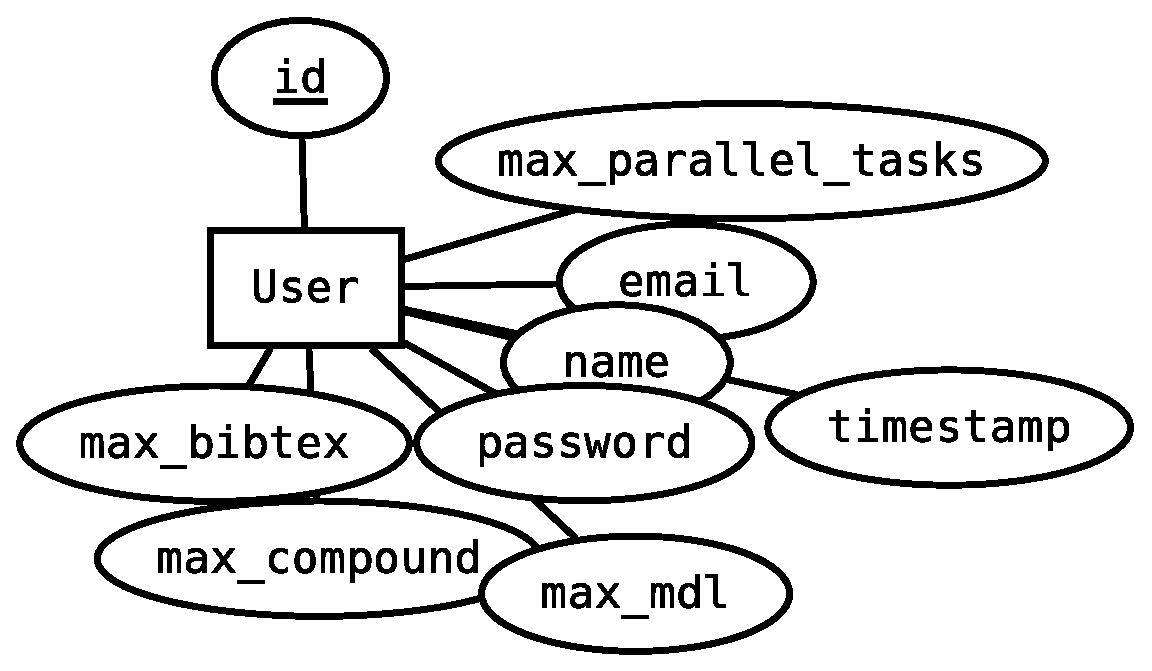
\includegraphics[keepaspectratio=true,width=0.55\textwidth]{figures/user}
\end{figure}

\subsection{Task and Error Report}
A task is identified by its ID. It has a status (running, queued,
cancelled, etc), percentage of completion, duration to complete (when
it has completed), URI of the result, corresponding HTTP status, 
and also points to the User who created it in the first place, 
as well as a creation timestamp. In case of an exceptional 
event, it links to an ErrorReport entity. This has an error code
(internal), HTTP status, debugging details, error message, 
actor (who is to blame for the exception), and an identifying ID.

\begin{figure}[h]
 \centering
 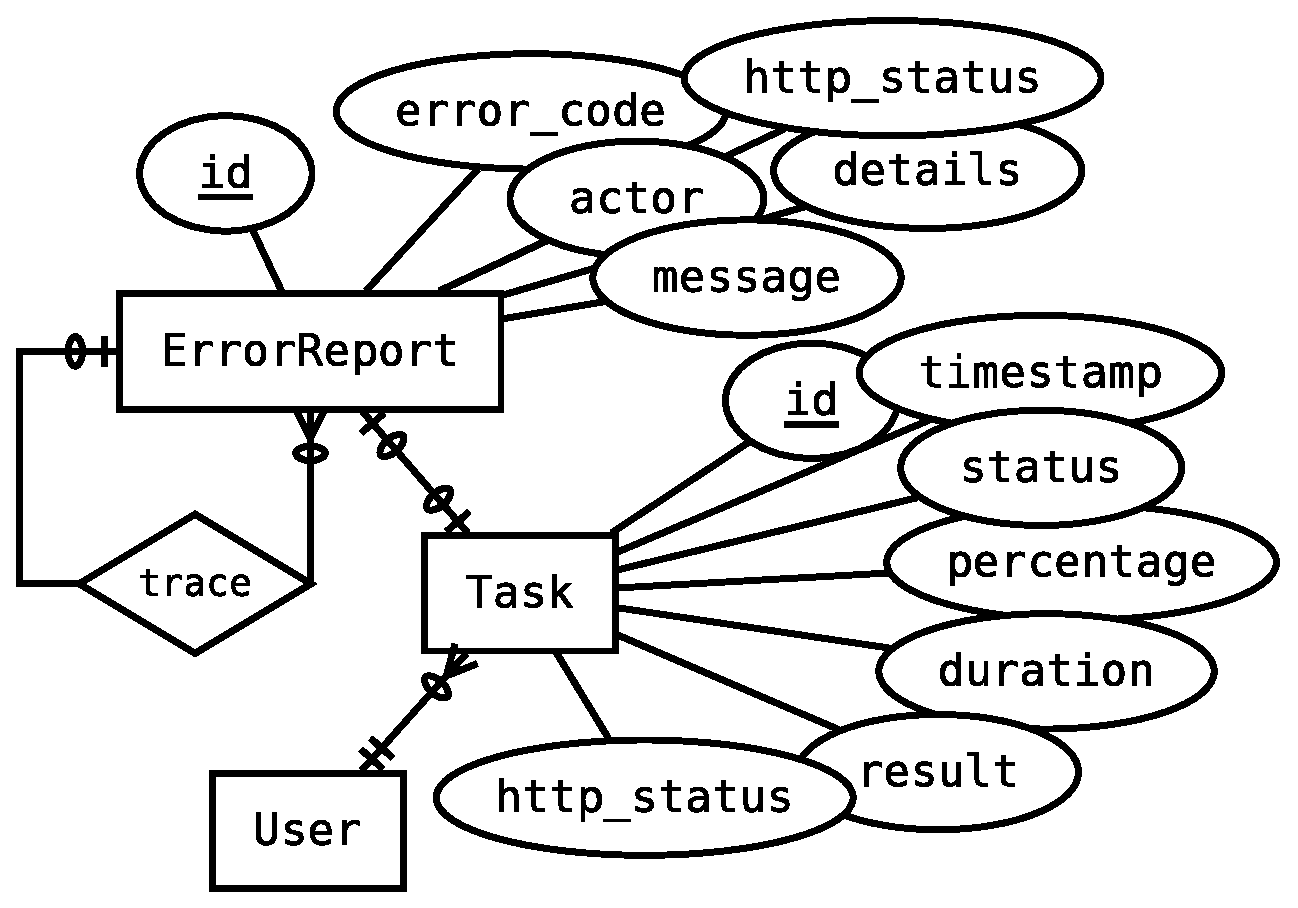
\includegraphics[keepaspectratio=true,width=0.6\textwidth]{figures/task_error}
\end{figure}


\subsection{Substance}
Substance is a central figure in JAQPOT: A Substance can be either a
chemical Conformer or a Nanomaterial, while in the future other classes
may be added (e.g., proteins, DNA, etc.). A Substance from JAQPOT's
perspective is (i) what identifies a \textit{row} in a \textit{dataset} for
training and (ii) input for prediction using a model.
Substances are abstract entitied. In particular, in the current version, they
are subclassed by the distinct classes \texttt{Nanomaterial} and \texttt{Conformer}.

\subsection{Conformer}
A Conformer is a chemical compound with a particular 3D configuration.
Chemical conformers are groupped together by the same \texttt{Compound}.
Conformers are characterized by their IDs and their various representations
(SMILES, SDF, InChI, etc).

\begin{figure}[h]
 \centering
 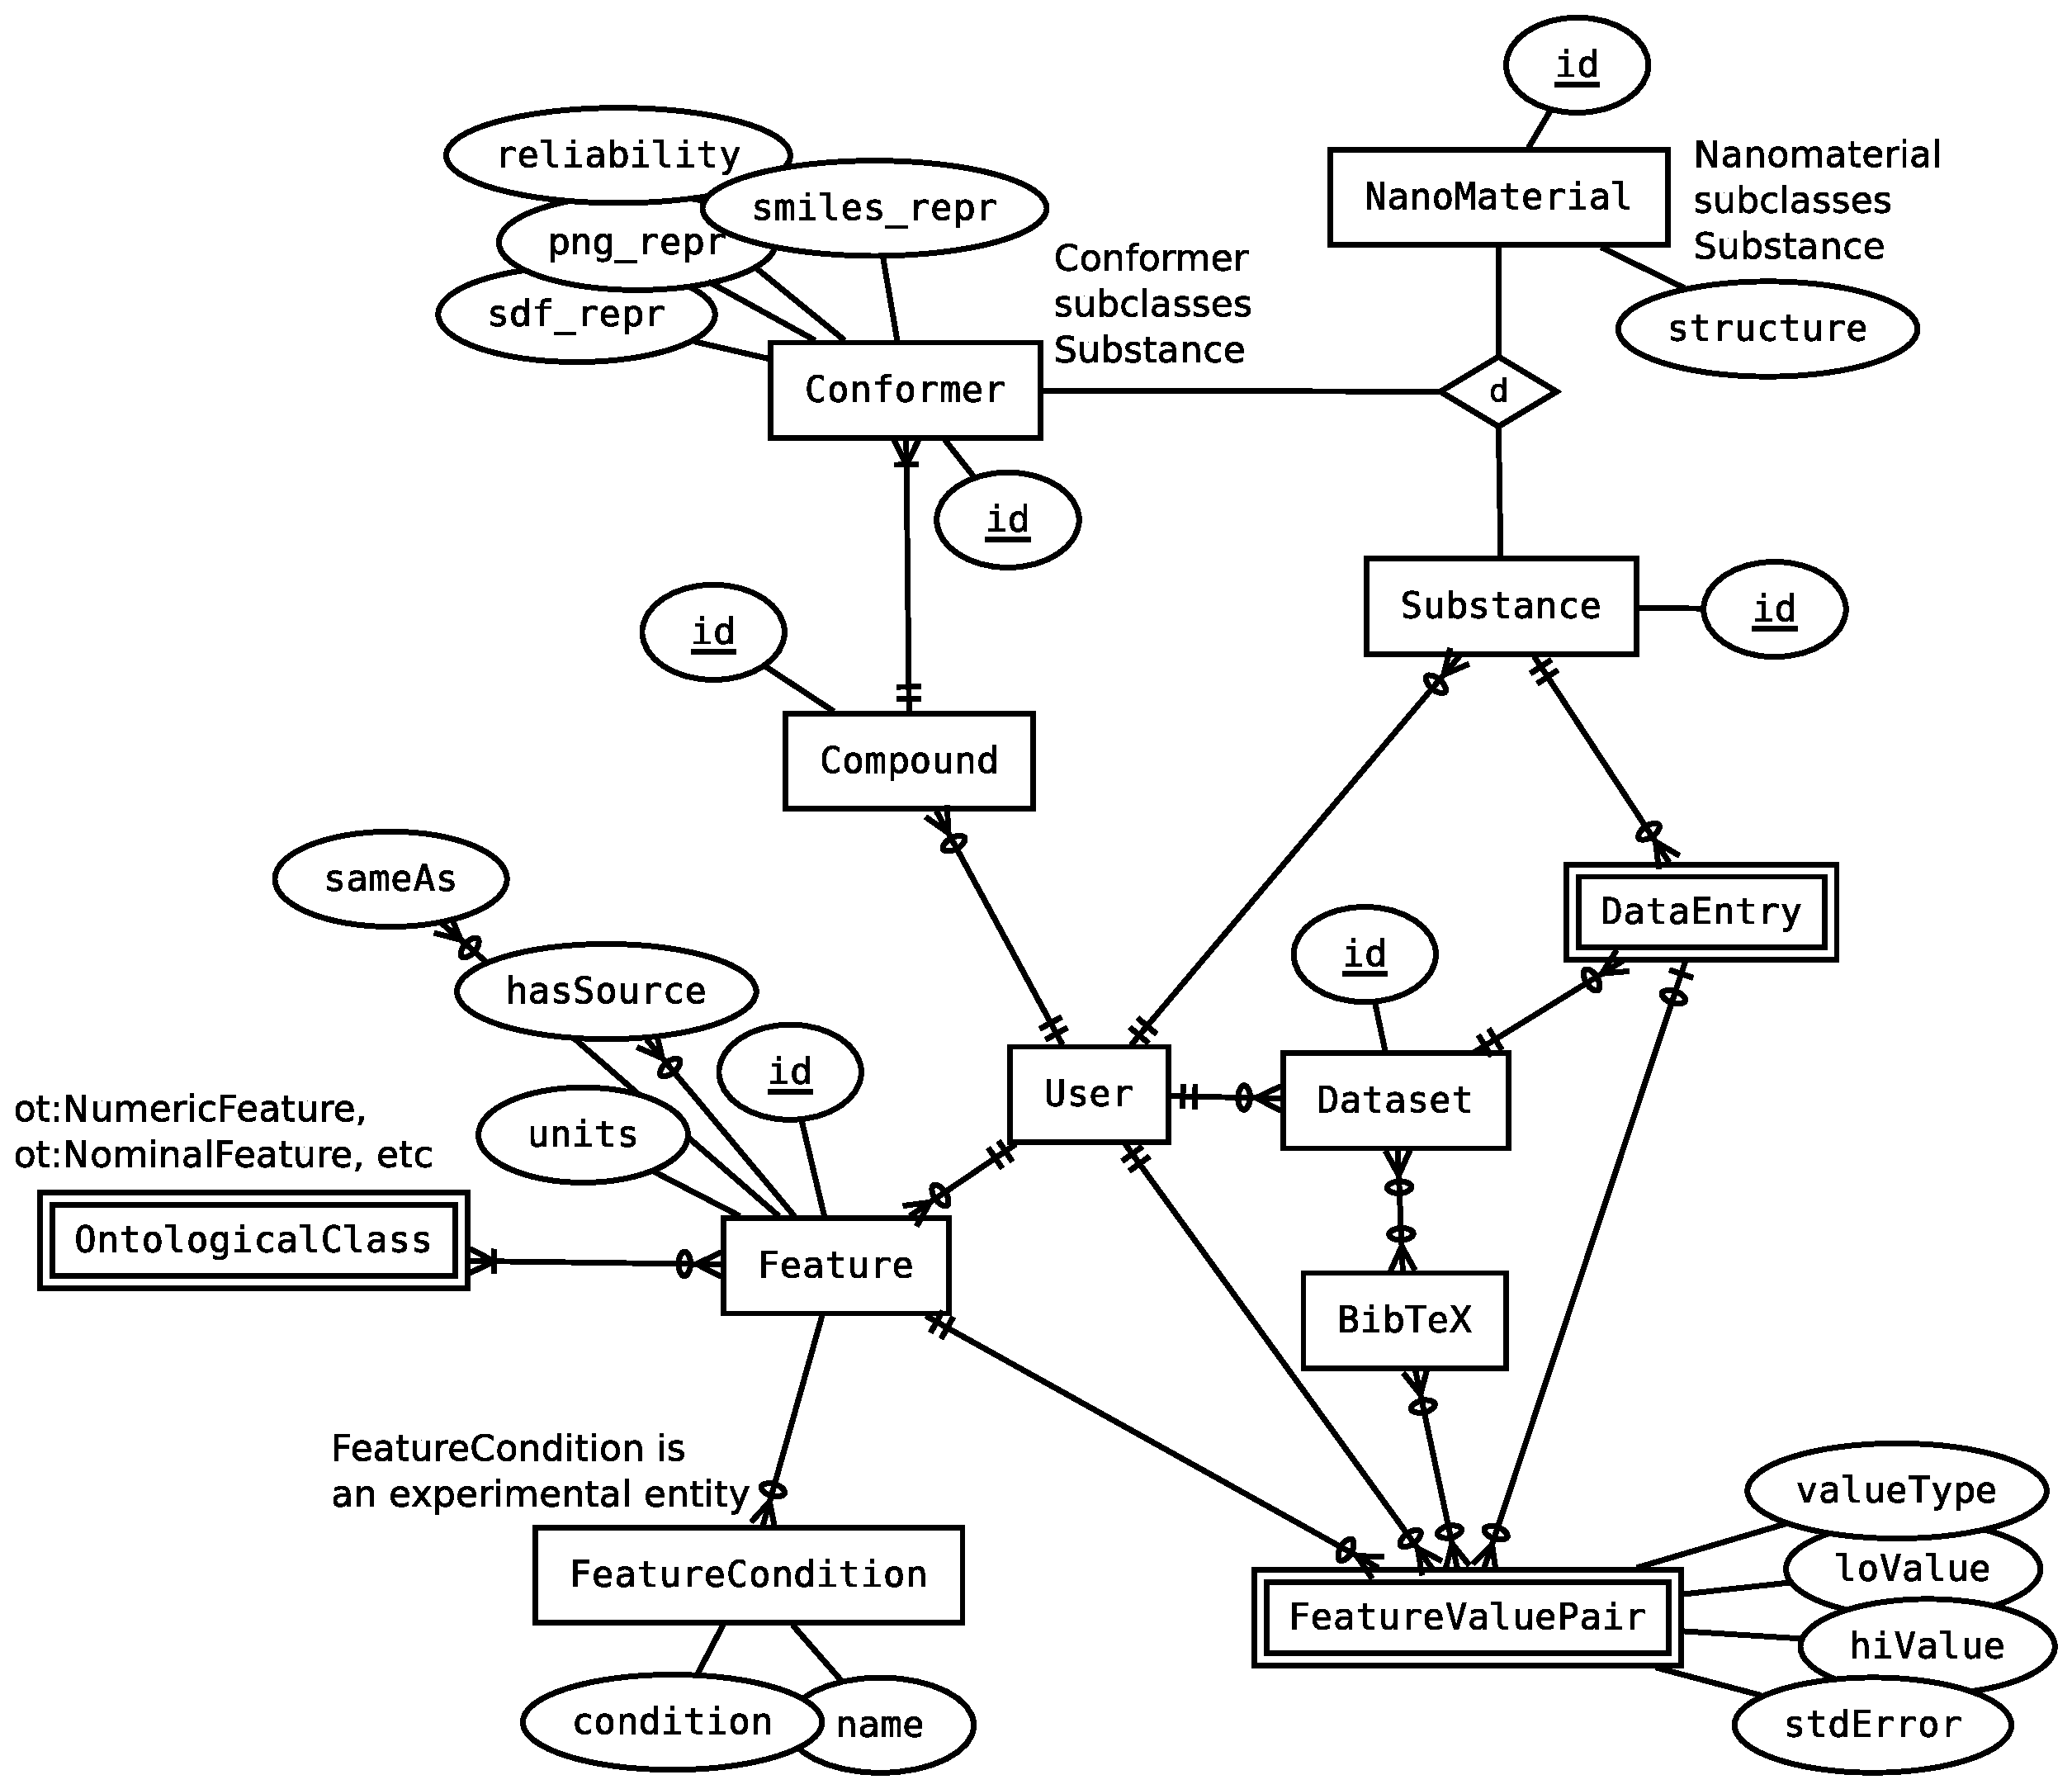
\includegraphics[keepaspectratio=true,width=0.8\textwidth]{figures/chemical_data}
\end{figure}

\subsection{Nanomaterials}
A nanomaterial is a particular instance of a Substance. Nanomaterials'
structure is described by the NPO ontology (http://www.nano-ontology.org/).



\subsection{Feature}
Features are properties that can be assigned to substances. The type of
a feature is determined by a link to an ontological class. For instance
a feature can be \texttt{ot:NominalFeature} or \texttt{ot:NumericFeature}
etc. Different features may be groupped together via \texttt{FeatureCondition}s.
Features possess also an ontological characterisation that can be 
used to search for them. When the feature can be computed \textit{in silico}
its \texttt{hasSource} attribute
is a link to the algorithm or model that can be used to compute it.


\subsection{FeatureValuePair}
A \texttt{FeatureValuePair} is exactly what its name implies: 
an feature-value pair in the database
for a particular substance and a given feature.
A Feature value pair may be part of a \texttt{DataEntry} whic is 
the elementary component of a Dataset. This entity has a lower
and a higher bound (in case it is single-valued, by convention,
\texttt{loValue} stores the value and \texttt{hiValue} is set to 
\texttt{null}. It has a value type (numeric, double, integer, 
etc), an error estimation (\textit{e.g.}, \texttt{stdError}).


\subsection{DataEntry and Dataset}
A data entry is simply a \textit{row} in a dataset;
there is a single substance (chemical conformer or nanomaterial) to which
the DataEntry pertains to. A Dataset is chiefly a collection of 
DataEntry entities. 



\subsection{Algorithm}
\lipsum[1]

\begin{figure}[h]
 \centering
 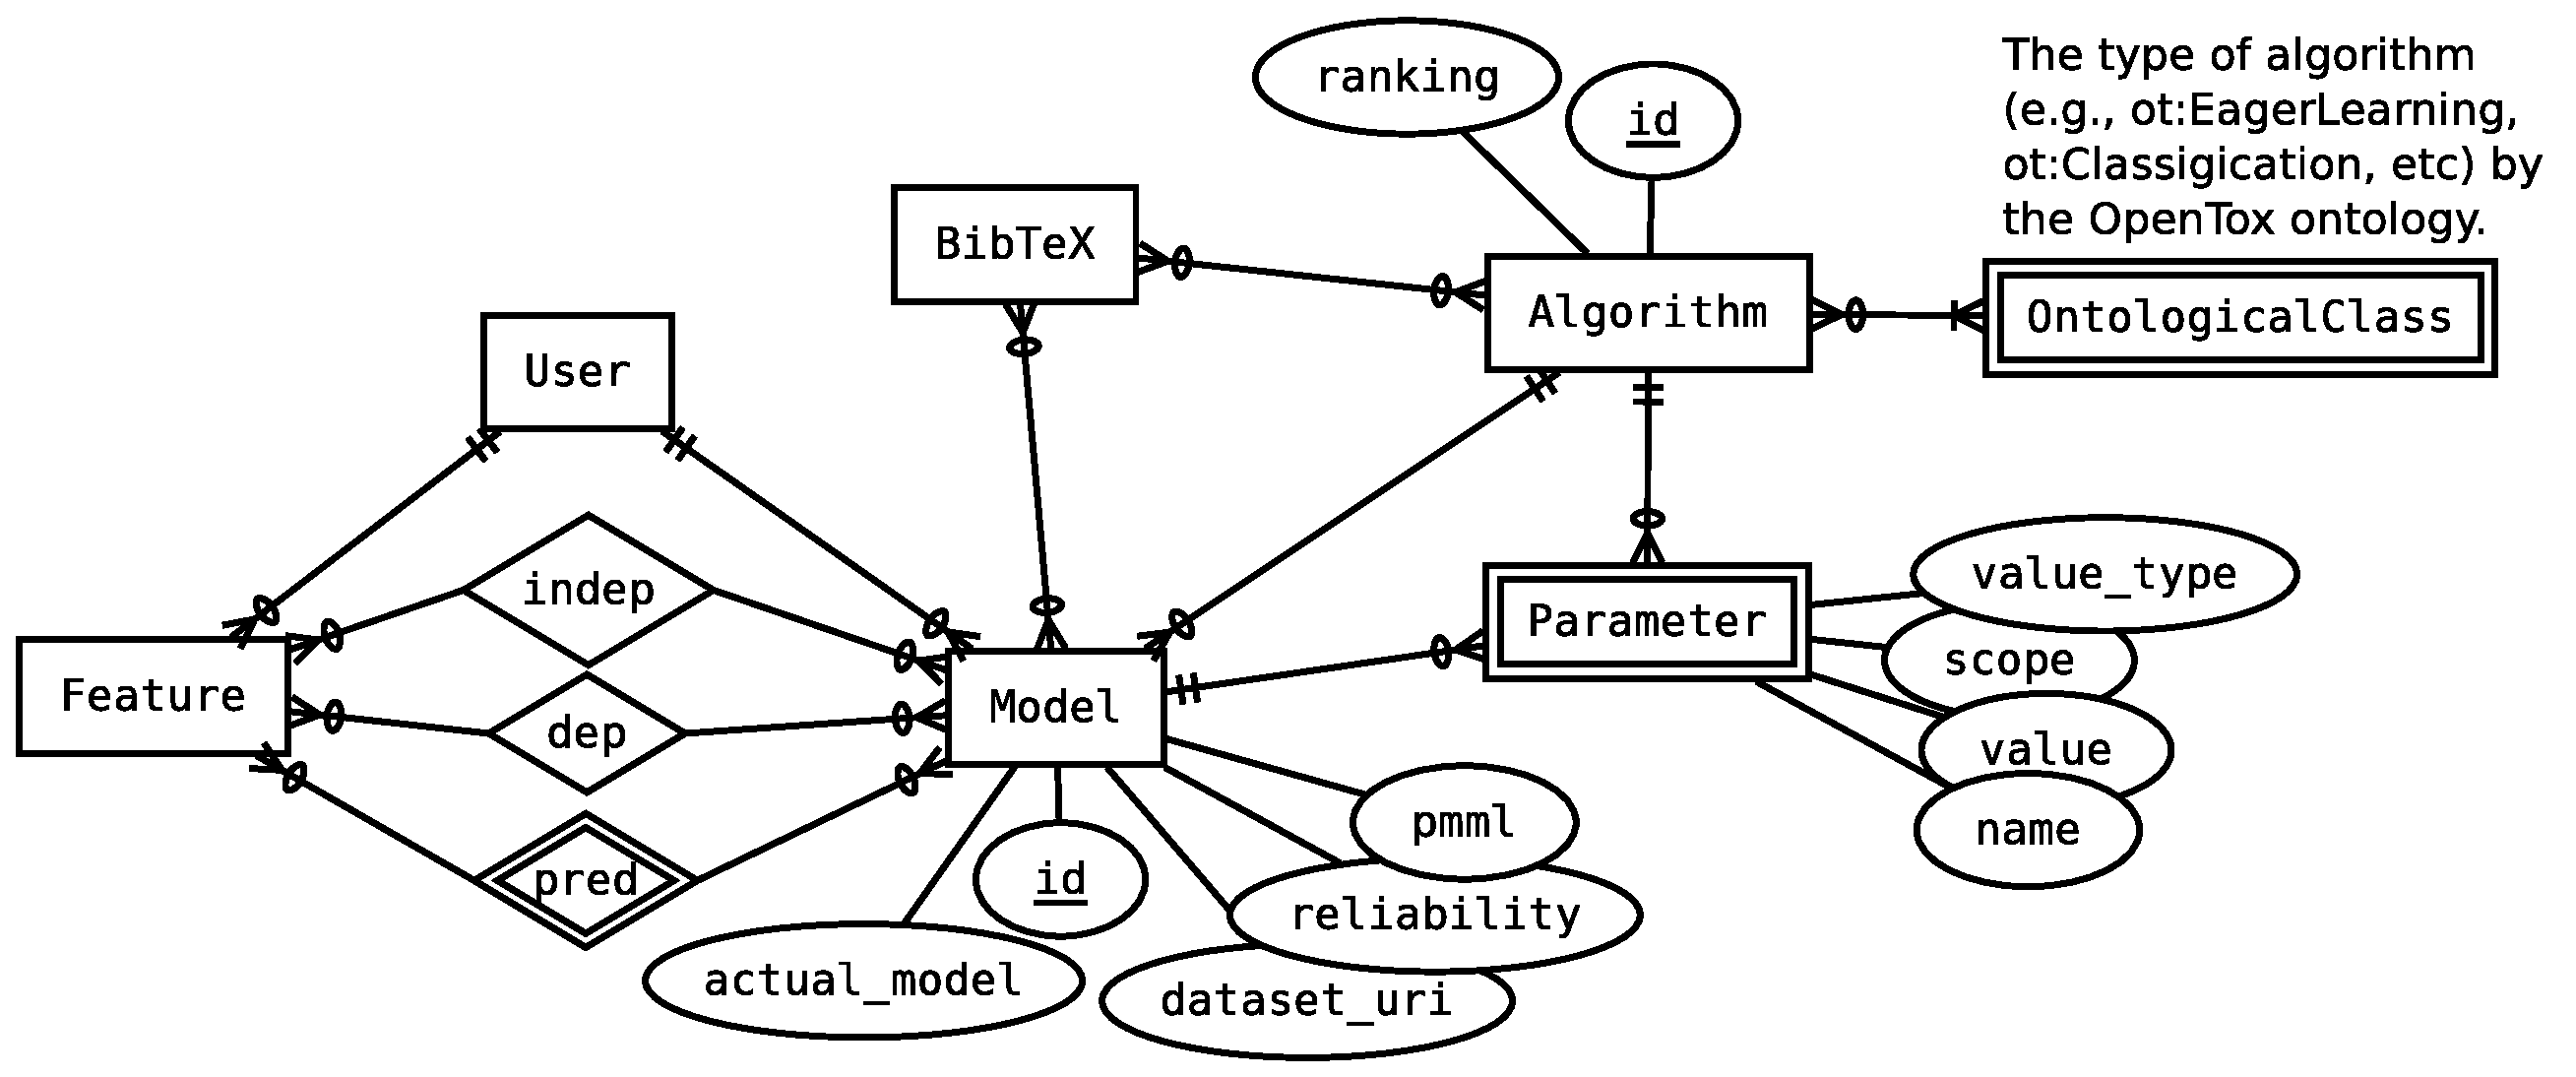
\includegraphics[keepaspectratio=true,width=0.95\textwidth]{figures/model_algorithm}
\end{figure}

\subsection{Model}
\lipsum[2]